%%%%%%%%%%%%%%%%%%%%%%%%%%%%%%%%%%%%%%%%%%%%%%%%%%%%%%
%
% This file defines the style for your report
% You don't need to edit it any more, if not to change the authors name.
%
% Search below for the keyword:   GROUP
% insert your group number
%
% Search below for the keyword:   AUTHORS
% insert the name of the authors
%
% If you want to compile your document you have TWO ways
% depending on the fact that 
% 	1) you have inserted only postscript images in your .tex file 
%		---> then go to MODE 1
%	2) you have inserted other kind of images (jpg, pdf, ...) in your .tex file
%		---> then go to MODE 2
%
% MODE 1 
% Type:
% 	latex homebook.tex
%
% If the compilation runs successfully and you want to see the results type:
% 	xdvi homebook.dvi &
% and use the menus to go through the document
%
% If you want to create a pdf type:
% 	dvipdfm homebook.dvi
%
% a homebook.pdf file is created
% you can see it using the command:
% 	acroread homebook.pdf &
%
%
% MODE 2
% Type:
%	pdflatex homebook.tex
%
% If the compilation runs successfully you directly have the pdf file
% and you can see it using the command:
%       acroread homebook.pdf &
%
% 
%%%%%%%%%%%%%%%%%%%%%%%%%%%%%%%%%%%%%%%%%%%%%%%%%%%%%%

\documentclass[12pt,  english, makeidx, a4paper, titlepage, oneside]{book}
\usepackage{babel}
\usepackage{fancyhdr}
\usepackage{makeidx}
\usepackage{titlesec}
\usepackage{listings}
\usepackage{booktabs}

\newenvironment{listato}{\footnotesize}{\normalsize }

%\pagestyle{empty}

\textwidth 15.5cm
\textheight 23cm
\topmargin -1cm
\oddsidemargin -0.5cm
\linespread{1.1}

\pagestyle{fancy}
\fancypagestyle{plain}{%
	\fancyfoot[LE, RO]{\textcopyright \textit{Garolla, Jiang, Forno, Buttafuoco, Bellino\\
		Project 8 - IP-core Manager for FPGA-based Designs (RT level)}} %dx
	\fancyfoot[LO, RE]{}} %sx
\lhead{}
%\chead{System design project} %MODIFICARE IL NOME
\rhead{}
\lfoot{}
\cfoot{}
\rfoot{ \textcopyright \textit{Garolla, Jiang, Forno, Buttafuoco, Bellino\\
	Project 8 - IP-core Manager for FPGA-based Designs (RT level)}}%MODIFCARE
\rhead{\thepage}
%\usepackage{minted}
\usepackage{graphicx}
\usepackage{amsmath}
\usepackage{amsfonts}
\usepackage{amsthm}
\usepackage{amssymb}
%\oddsidemargin -1.1cm
\usepackage{graphicx}
\usepackage{caption}
\usepackage{float}
\usepackage{amsmath}
\usepackage{amssymb}
\usepackage{amsfonts}
\usepackage{amsthm}
\usepackage{subscript}
\usepackage{empheq}
\usepackage{verbatim}
\usepackage{fancyvrb}
\usepackage{datetime}
\usepackage{hyperref}
\usepackage{color}
\hypersetup{%
	pdfpagemode={UseOutlines},
	bookmarksopen,
	pdfstartview={FitH},
	colorlinks,
	linkcolor={blue},
	citecolor={red},
	urlcolor={blue}
}
\definecolor{dkgreen}{rgb}{0,0.6,0}
\definecolor{gray}{rgb}{0.5,0.5,0.5}
\definecolor{mauve}{rgb}{0.58,0,0.82}

\lstset{frame=tb,
	language=VHDL,
	aboveskip=3mm,
	belowskip=3mm,
	showstringspaces=false,
	columns=flexible,
	basicstyle={\small\ttfamily},
	numbers=left,
	numbersep=5pt,
	numberstyle=\tiny\color{gray},
	keywordstyle=\color{blue},
	commentstyle=\color{dkgreen},
	stringstyle=\color{mauve},
	breaklines=true,
	breakatwhitespace=true,
	tabsize=3
}


\titleformat{\chapter}[display]
{\normalfont\Large\filcenter\sffamily}
{\titlerule[0.5pt]%
\vspace{1pt}
\titlerule
\vspace{1pc}
\LARGE\MakeUppercase{\chaptertitlename} \thechapter
}
{1pc}
{\titlerule
\vspace{1pc}
\Huge}
{}

\makeindex

\begin{document}

\frontmatter
\begin{titlepage}
\vspace{0cm}
\centerline{

\includegraphics[width=3cm]{./logopoli}} 
\vspace{0.5cm}
\centerline{\LARGE Politecnico di Torino}
\vspace{2cm}
\centerline{\Huge\sf System design project}
\vspace{1cm}
\centerline{\huge \sf Project8 }
\bigskip
\centerline{\huge\sf IP-core Manager for FPGA-based Designs (RT level)}
\bigskip
\centerline{\huge\sf Final Report}
\vspace{1.5cm}
\centerline{\Large Master degree in Computer Engineering}
\centerline{\Large Specialization in Embedded Systems}
\bigskip
\vspace{0.5cm}
%%%%%%%%%%%%%%%%%%%%%%%%%%%%%%%%%%%%%%%%%%%%%%%%%%%%%%
%
\centerline{\large Referents: }
\centerline{\large Prof. Paolo Ernesto Prinetto}
\centerline{\large PhD. Student Giuseppe Air\`{o} Farulla}
\bigskip
\vspace{0.5cm}
%
%%%%%%%%%%%%%%%%%%%%%%%%%%%%%%%%%%%%%%%%%%%%%%%%%%%%%%
% GROUP
% Change the name of your group below
%
\centerline{\large Authors:}
\bigskip
%
%%%%%%%%%%%%%%%%%%%%%%%%%%%%%%%%%%%%%%%%%%%%%%%%%%%%%%
% AUTHORS
% Change the name of the Group participants here
%
\centerline{\large Emanuele Garolla}
\centerline{\large Gina Jiang}
\centerline{\large Evelina Forno}
\centerline{\large Francesco Buttafuoco}
\centerline{\large Salvatore Bellino}

%
%%%%%%%%%%%%%%%%%%%%%%%%%%%%%%%%%%%%%%%%%%%%%%%%%%%%%%
\vspace{1.5cm}
\newdateformat{monthyeardate}{%
	\monthname[\THEMONTH], \THEYEAR}
\centerline{\large \monthyeardate\today}
\end{titlepage}
 %\include{content/frontmatter/acknowledgements}
 
\newenvironment{acknowledgements}%
{\cleardoublepage\thispagestyle{empty}\null\vfill\begin{center}%
		\bfseries\textbf{ \huge Acknowledgements}\end{center}}%
{\vfill\null}

\section*{}
\bigskip
\bigskip
\begin{center}
	{\huge \textbf{Acknowledgement}}
\end{center}
\bigskip
We would like to express our special thanks of gratitude to our class mates involved in a similar project (project 14, 7 and especially 13) who collaborated with us on defining the CPU On Board IP-core Manager protocol.

\tableofcontents

\mainmatter
%%%%%%%%%%%%%%%%%%%%%%%%%%%%%%%%%%%%%%%%%%%%%%%%%%%%%%
%    
% HERE IS WHERE YOU INCLUDE YOUR CHAPTERS
%
%%%%%%%%%%%%%%%%%%%%%%%%%%%%%%%%%%%%%%%%%%%%%%%%%%%%
% This will help you in writing your homebook
% Remember that the character % is a comment in latex
%
% chapter 1

%%%%%%%%%%%%%%%%%%%%%%%%%%%%%%%%%%%%%%%%%%%%%%%%%%%%%%%%%%%
% you can organize a chapter using sections -> \section{Simulating an inverter}
% or subsections -> \subsection{simulating a particular type of inverter}

%%%%%%   First section

\chapter{Report on the activities held}
\begin{table}[h]
	\begin{tabular}{p{2.1cm}|  p{13.5cm}}
\multicolumn{2}{p{15.0cm}}{ \LARGE{{Setting up the group and the environment to work in team}}}\\
\hline \hline 
\multicolumn{2}{p{1.0cm}}{ \Large{{}}}\\
	07/03/2017 & \textbf{Group formation and selecting the homework}\\
	12/03/2017& Discussing the possibility to work in a team of 4 people, and the preference of the homework available. \\
	\multicolumn{2}{p{1.0cm}}{ \Large{{ }}}\\	
	15/03/2017 & \textbf{Confirmation of the group}	 \\
	&It has been announced the groups and the related project. Another member joined the team. \\
	&We also exchanged the email address and the telephone number to fasten the communication between members abroad (Whatsapp, Skype, Telegram...).\\
		\multicolumn{2}{p{1.0cm}}{ \Large{{ }}}\\
		22/03/2017 & \textbf{Redmine platform}\\
		27/03/2017& Set-up the Redmine platform. Understanding how to use it, register, open a new topic, upload file, register time. \\
		\multicolumn{2}{p{1.0cm}}{ \Large{{ }}}\\	

\end{tabular}
\end{table}	
\begin{table}[h]
	\begin{tabular}{p{1.9cm}|  p{13.5cm}}	
	\multicolumn{2}{p{15.0cm}}{ \LARGE{{Understanding the environment and the requirements}}}\\
	\hline \hline 
	\multicolumn{2}{p{1.0cm}}{ \Large{{}}}\\
	22/03/2017 & \textbf{SEcube documentation}\\
	03/04/2017& Reading the SEcube documentation and write down the analysis.\\
	\multicolumn{2}{p{1.0cm}}{ \Large{{ }}}\\		
	03/04/2017 & \textbf{Communication Protocol v.1.0}\\
	10/04/2017& Meeting with the professor on $ 3^{rd} $ April and on $ 4^{th} $ April. Then we discussed with other projects team (project 13, 7, 14) to enhance the protocol.
	\\ \multicolumn{2}{p{1.0cm}}{ \Large{{ }}}\\	
		11/04/2017 & \textbf{Communication Protocol v.2.0}\\
		20/04/2017 & During Easter Holyday, the project 13 sent the second version to the teacher, but other modifications were needed.\\
		\multicolumn{2}{p{1.0cm}}{ \Large{{ }}}\\	
		26/04/2017 & \textbf{Communication Protocol v.3.0}\\
		02/05/2017 & Discussion with the team involved. Then the project 13 submitted the final protocol.
\end{tabular}
\end{table}	
\begin{table}
	\begin{tabular}{p{2.1cm}|  p{13.5cm}}
		\multicolumn{2}{p{15.0cm}}{ \LARGE{{Project Development and Documentation}}}\\
		\hline \hline 
		\multicolumn{2}{p{1.0cm}}{ \Large{{}}}\\
		18/04/2017 & \textbf{GIT setup and backbone in VHDL}\\
		23/04/2017& Read GIT manual, GIT set up.\\
		 &Write in VHDL the interface of all the components.\\
		\multicolumn{2}{p{1.0cm}}{ \Large{{ }}}\\	
		21/04/2017 & \textbf{Presentation of the $ 26^{th} $ April}	 \\
		26/04/2017 & It has been requested 3 slides talking about:\\
		& \quad- Gantt\\
			&\quad- Milestones - Deliverables\\
			&\quad- Issues already closed - still open..\\

	\multicolumn{2}{p{1.0cm}}{ \Large{{}}}\\
		02/05/2017 & \textbf{Developemnt of the IP-core Manager and documentation}\\
		10/06/2017&-Split the work among us\\
			& - Deciding the communication among the components\\
			& - Write down the architecture, upload it on GIT, perform some tests\\
			& - Report timing and area and synthesys results with LATTICE Diamond\\
			& - Documentation and presentation\\
	%	10/06/2017& We discussed how to split the work among us, if there were any problem between the communication between some components.\\
	%	&We then wrote the architecure in VHDL, upload it on GIT, do some test, write some documentations and presentation.\\
	%	&Finally we tried to some synthesys on the LATTICE Diamond software and tried to the source file on the board.\\
		\multicolumn{2}{p{1.0cm}}{ \Large{{ }}}\\	
		
	\end{tabular}
\end{table}

\begin{figure}[h!]
	\centering	
	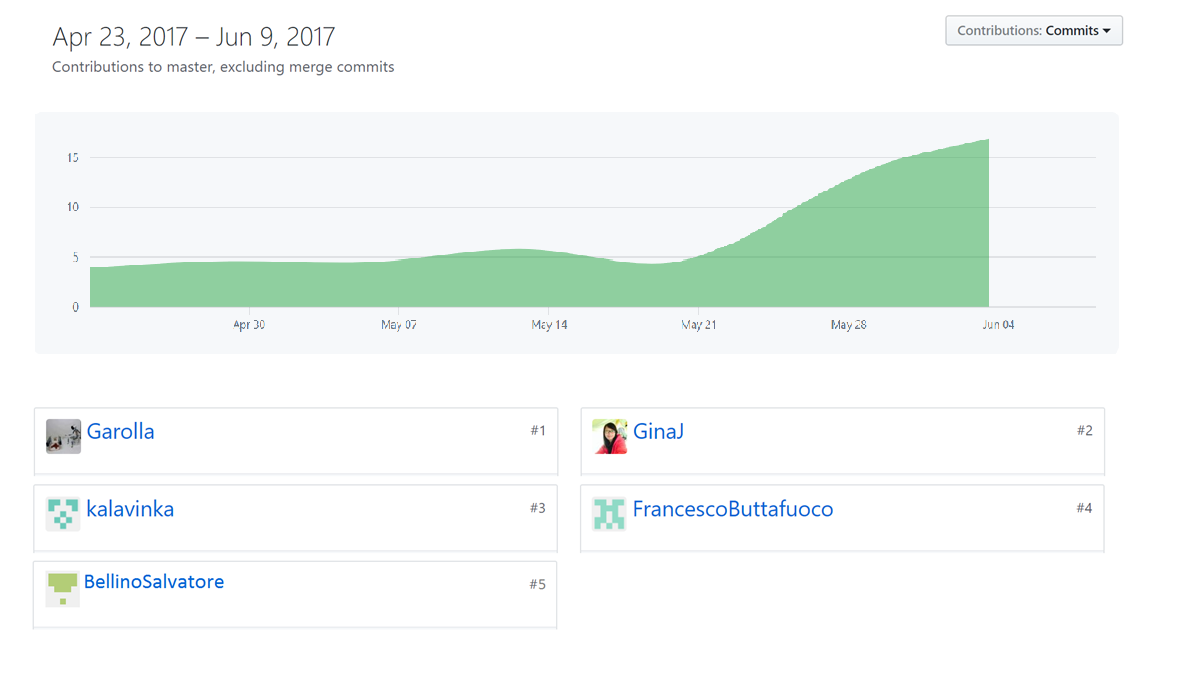
\includegraphics[width=\textwidth]{chapters/git.png}  
	\caption{Our project on GIT, with us as contributors} 
	\label{git}
\end{figure}	
\begin{table}
	\begin{tabular}{p{3.5cm}|  p{12.1cm}}
		\multicolumn{2}{p{15.0cm}}{ \LARGE{{Assignment of the tasks }}}\\
		\hline \hline 
		\multicolumn{2}{p{1.0cm}}{ \Large{{}}}\\
		GAROLLA Emanuele& -Backbone of project in VHDL\\
		& -Dual port buffer 64x16 (Behavioral)\\
		&-Assemble all files\\	
	 &-Final Testbench of the overall architecture	 \\
		 & -Slides\\
		
		\multicolumn{2}{p{1.0cm}}{ \Large{{}}}\\
		JIANG Gina& -Documentation for the $ 26^{th} $ April\\
		&-Documentation for the $ 27^{th} $ May\\
		&-Report timing and area, synthesys result (LATTICE Diamond)\\
		&-Technical report\\
		\multicolumn{2}{p{1.0cm}}{ \Large{{ }}}\\
		
		BELLINO Salvatore& -Dual port buffer 64x16 (Behavioral)\\
		&\qquad -Register 0\\
		&\qquad -Register 16 bits\\
		&\qquad -Decoder\\
		&-Testbench for the data buffer\\
		&-Slides	\\
			
%			\end{tabular}
%		\end{table}	
%		\begin{table}
%			\begin{tabular}{p{3.5cm}|  p{12.1cm}}
%					\multicolumn{2}{p{15.0cm}}{ \%LARGE{{Assignment of the tasks (part 2/2)}}}\\
%					\hline \hline
\multicolumn{2}{p{1.0cm}}{ \Large{{ }}}\\	
		FORNO Evelina& -Dummy IP-core\\
		&-Adder IP-core (FSM with 3 stage)\\
		&-First version of testbench\\
		&-Slides\\
		\multicolumn{2}{p{1.0cm}}{ \Large{{ }}}\\
		BUTTAFUOCO & -IP-Manager Behavioral\\
		Francesco&\qquad-Enabling the right IP core\\
		&\qquad-Propagate the right Data from the selected IP core to the Buffer/CPU\\
		&\qquad-Interrupt Handler\\
		&-Slides\\	
	\end{tabular}
\end{table}
\begin{figure}[h!]
	\centering	
	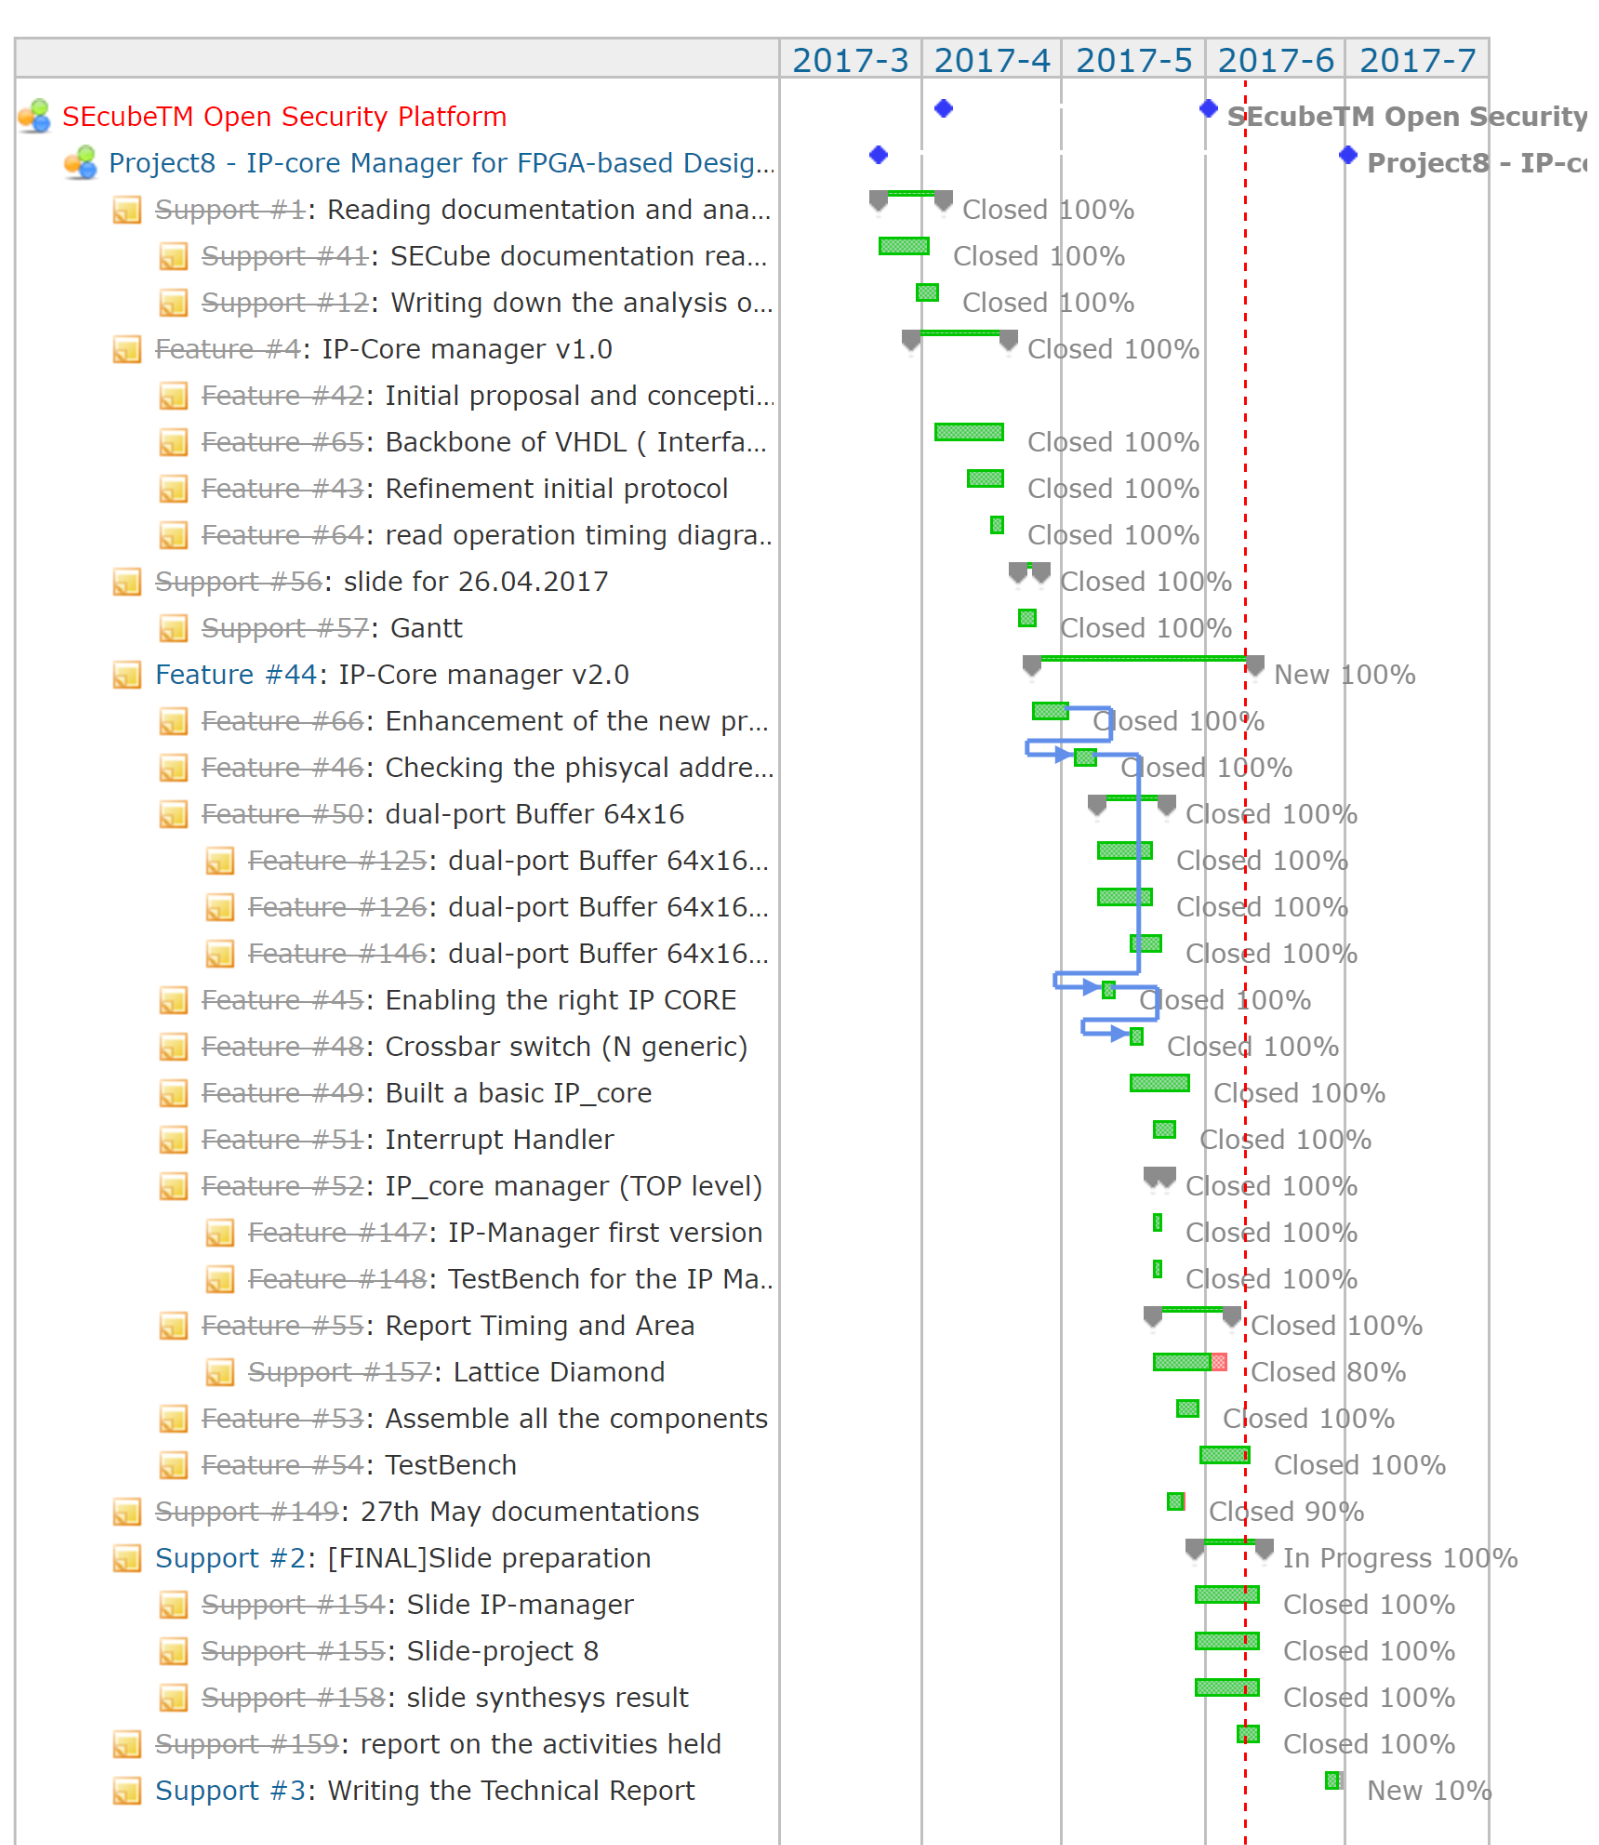
\includegraphics[height=0.65 \textheight]{chapters/gantt.png}  
	\caption{Gantt chart of our project} 
	\label{gantt}
\end{figure}	
\chapter{System's architecture}

\section{Components}
For this project, 3 main components are required (fig. \ref{00fig}):
\begin{enumerate}
	\item \textbf{IP-core Manager}:it's the main element of this architecture and its main goal is to handle the complexity of this system. It has to provide the correct exchange of data between the target IP-core and the CPU. Moreover it has to handle the interrupt service routine.
	\item \textbf{Data Buffer}:it's a dual port buffer that stores the data coming both from the CPU and the selected IP-core. It also enable the communication of the desired transaction from the CPU to the IP-core Manager by means of the $ row0 $ which is always read from the IP-core Manager
	\item \textbf{IP-core}:a core that perform a specific task or function.
\end{enumerate}
\section{Interfaces}

A multi IP-core system requires a IP core manager to handle the complexity of this system.
Main tasks of the IP Manager are the correct exchange of data between the target IP and the CPU. Another critical task is the interrupt handling. Figure \ref{00fig} shows the overall architecture of the whole system adopted.\\
	
	As shown in the figure \ref{00fig}, the IP manager indirectly communicates with the CPU through a dual port data buffer. This buffer has a standard interface and it is used to redirect data to/from the IP core selected.
	Whenever the CPU wants to start a transaction, it has to write some control bits (explained in section \ref{transaction}) at address 0 ($ row0 $) of the data buffer.
	The data in this address is always read from the IP Manager to speed-up the routing process whenever a new transaction begins.\\
\subsection{Data Buffer interface}\label{bufinter}
This data buffer has a standard interface.
The signals for this components (whether they come from the CPU or from from the IP core Manager of from both of them) has the following function: 
\begin{itemize}
	\item \textbf{data}: input/output port, used for transferring data from/to the CPU to/from the buffer. 
	\item \textbf{add}: input port, used for selecting the right row within the buffer to write/read data. 
	\item \textbf{w\_enable}: input port, must be asserted in order to enable write operation. 
		\item \textbf{w\_enable}: input port, must be asserted in order to enable read operation.  
		\item \textbf{generic\_enable}: input port, must be asserted in order to start any operation on that port. 
		\item \textbf{reset}: input port, it brings the buffer to the reset state. 
		\item \textbf{row\_0}: output port, it reflects any change in the row 0 of the buffer. 
\end{itemize}
\subsection{IP core interface} \label{IPinter}
	As for a generic $ x $ IP core interface, we have the following signals:
	\begin{itemize}
	\item \textbf{data\_in\_IPs(x)}:data from the $ x $ IP-core to the CPU/Data buffer.
\item \textbf{data\_out\_IPs(x)}:data to the $ x $ IP-core from the CPU/Data buffer.
\item \textbf{add\_IPs(x)}:address from the $ x $ IP-core to the Data buffer.
\item \textbf{W\_enable\_IPs(x)}: when the $ x $ IP-core wants to write to the buffer
\item \textbf{R\_enable\_IPs(x)}: when the $ x $ IP-core wants to read from the buffer
\item \textbf{Generic\_en\_IPs(x)}: when the $ x $ IP-core wants to communicate with the buffer	
\item \textbf{enable\_IPs(x)}: when the CPU wants to communicate with the $ x $ IP-core
\item \textbf{ack\_IPs(x)}: the IP-core manager sent this signal to the $ x $ IP-core to tell it that its interrupt request will be served
\item \textbf{interrupt\_IPs(x)}: when the $ x $ IP-core raises an interrupt request
\end{itemize}
	\begin{figure}[h]
		\centering
		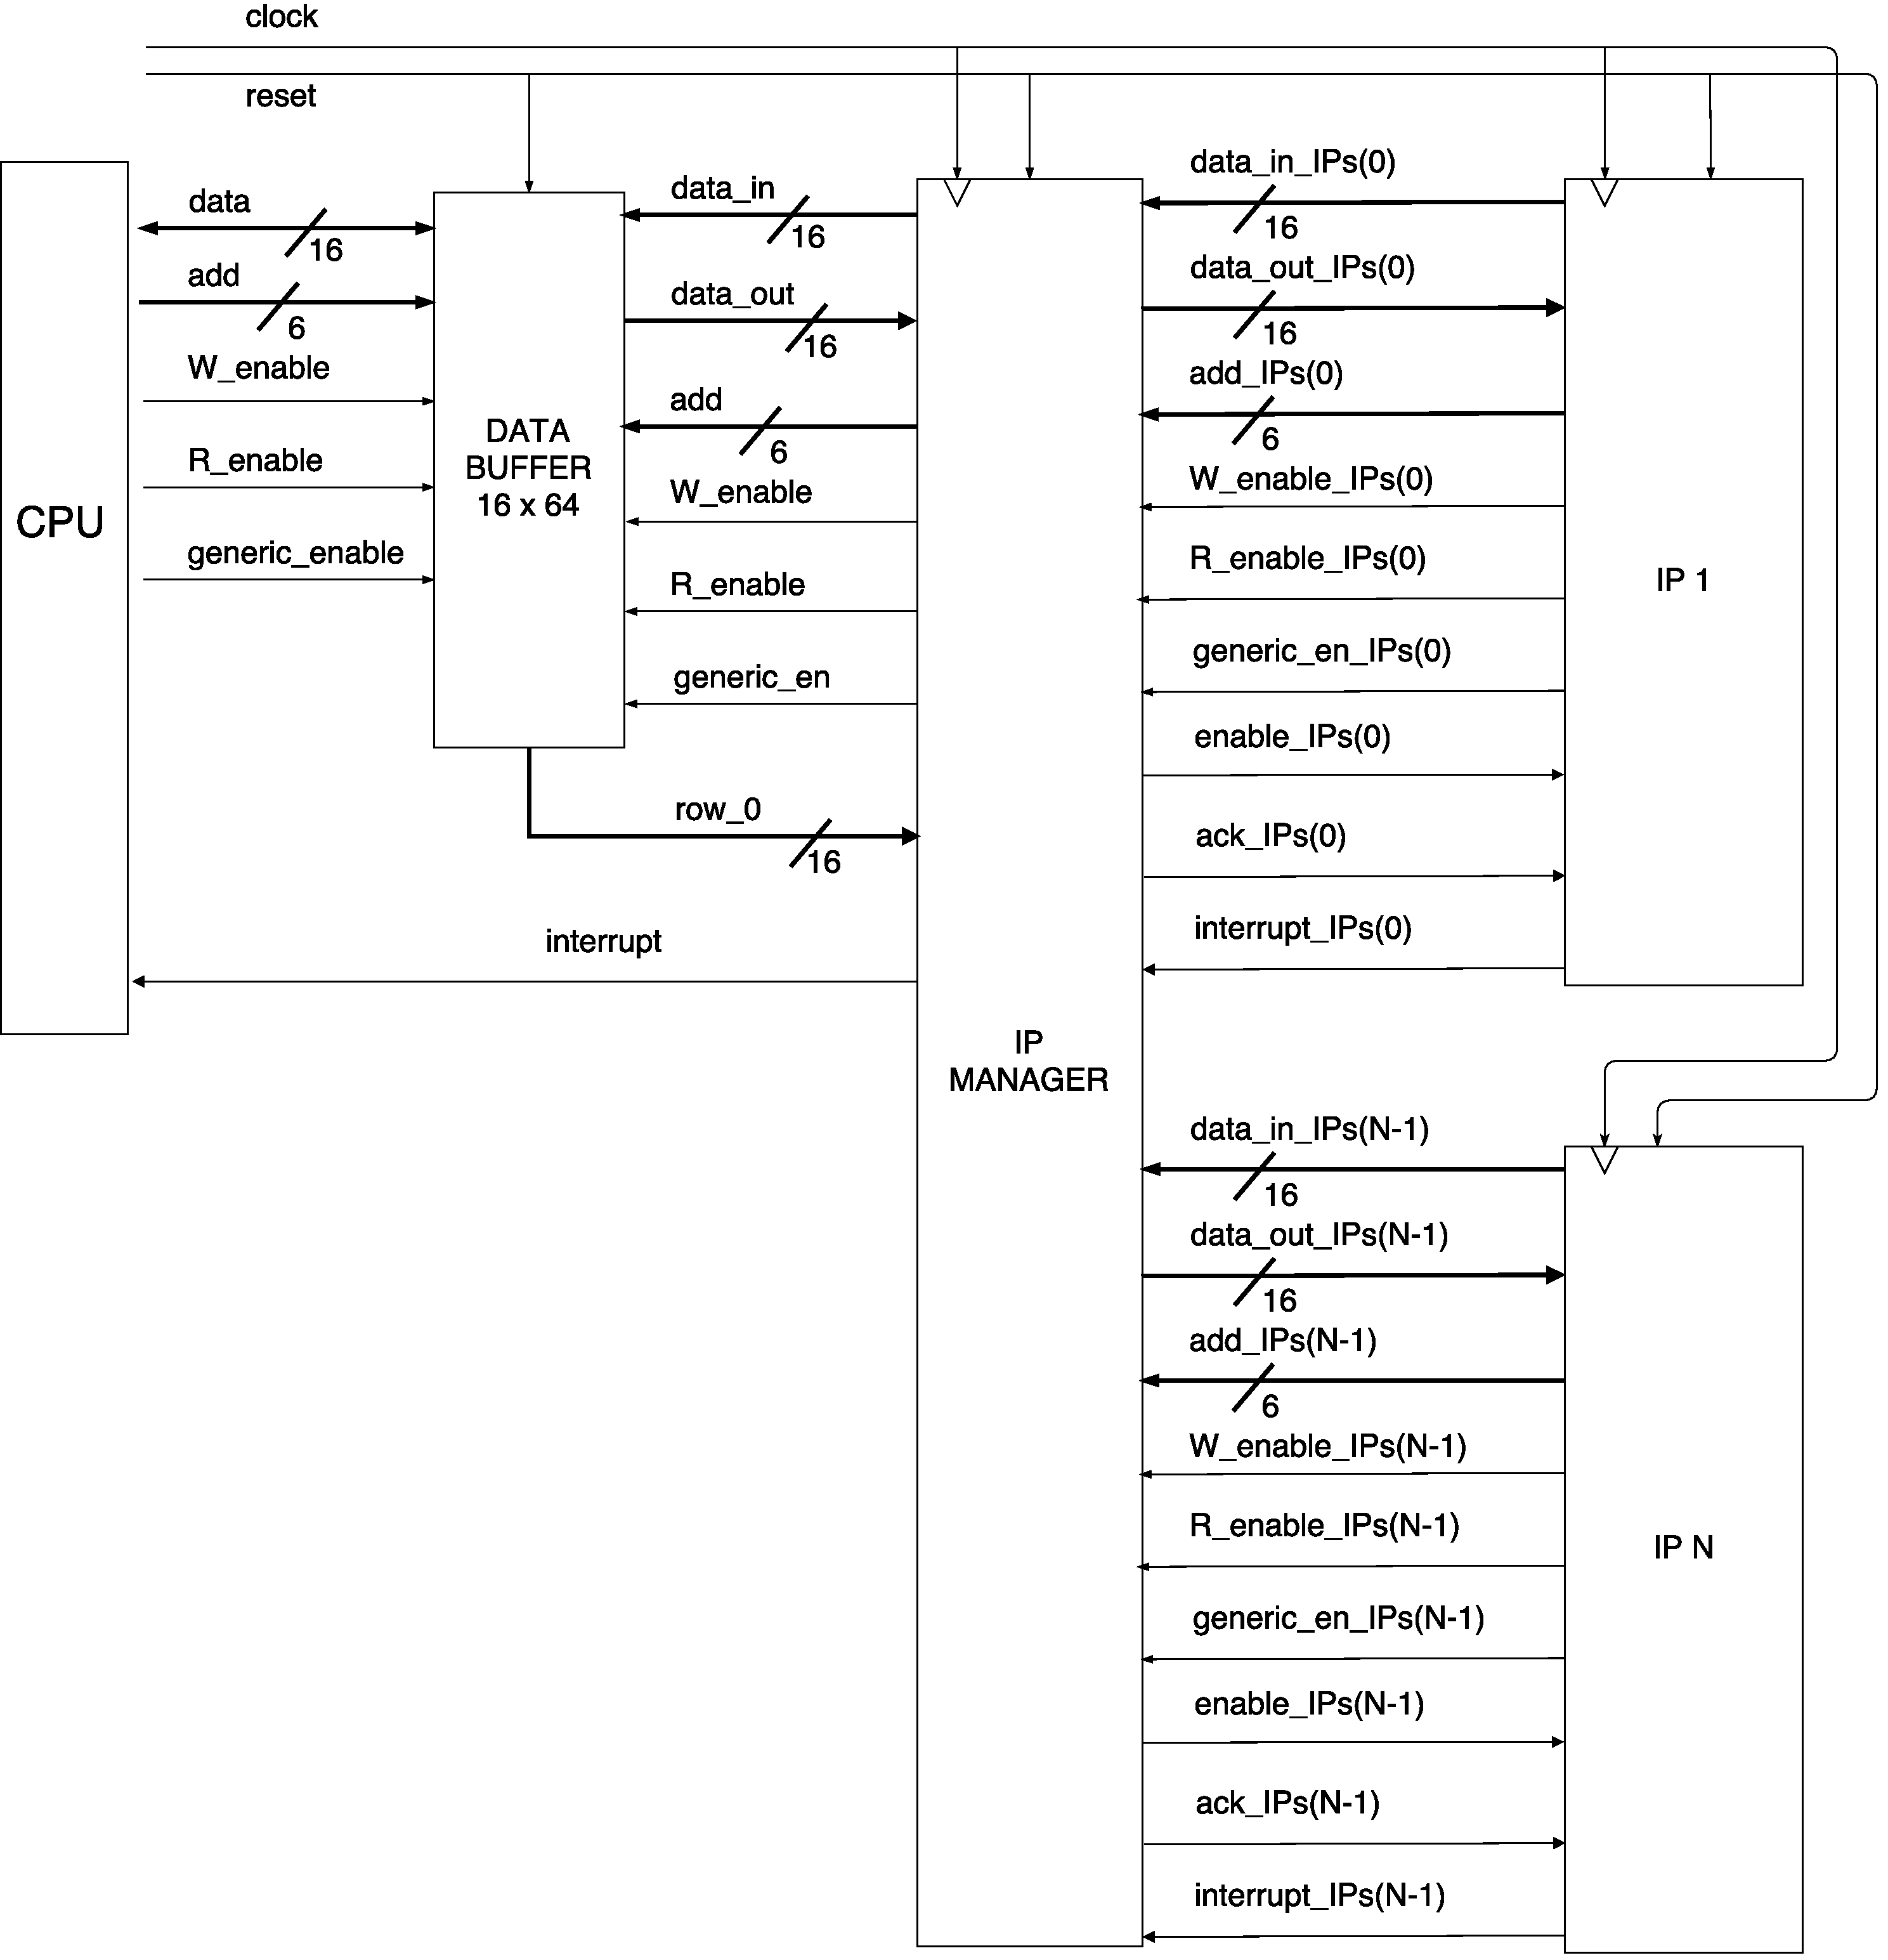
\includegraphics[width=0.95\textwidth]{chapters/figures/Interface.pdf}  
		\caption{System architecture}
		\label{00fig}
	\end{figure}
\clearpage
\newpage
\section{CPU Control bits } \label{transaction}

	When the CPU wants to start a transaction, it has to write a data packet with the following structure\\
	\begin{center}
	\begin{tabular}{ | l | l |  l | l | }
		
		15  \qquad  \qquad 14 & 13 & 12 & 11 \qquad \qquad 0 \\ \hline
		UNUSED & INT & B/E & IP ADDR\\ \hline
		
		
		\hline
	\end{tabular}
\end{center}

\bigskip
\begin{center}
	\begin{tabular}{ | c | p{7 cm} |  l |}
		\hline
		Bit(s) & Purpose & Value(s)  \\ \hline
		Bit 15 & unused  & unused 
		\\ \hline
		Bit 14 & unused  & unused\\
		\hline
		Bit 13 & Interrupt ACK from the CPU   & Normal = 0, Interrupt  =  1
		\\ \hline
		
		Bit 12 & Signals the begin/end of a transaction & Begin  = 1, End = 0 
		\\ \hline
			
		
			
		Bit 11-0 & The physical address of the target IP &
		From 0 up to N-1  \\
		
		
		
		\hline
	\end{tabular}
\end{center}
For a better understanding of the transaction mechanism, please see chapter \ref{usecase}.

\chapter{IP-core Manager functionalities}
\label{chap1}
\section{Enabling the right IP}
The first and basic task for this core manager is to enable the connection between the CPU and the selected core. More in particular this means exchanging the data in the required time as described in the protocol. The CPU can talk to one and only one core, therefore the core manager will disregard other cores whether they finished or not their task.
We know that the CPU writes at $ row_{0} $ what it wants to do. Here we can read the physical address of the chosen IP core.
If we know that the $ 1^{st} $ core is selected, than the IP manager has to enable the $ 1^{st} $ core (i.e. $port_{0}  $) and disable all the other ones, thus having the following signal:\\
\begin{center}
	$ enable_0='1' $\\
$ enable_1='0' $\\
$ enable_2='0' $\\
$  \vdots $\\
$ enable_{n-1}='0' $
\end{center}
\bigskip
We can put all these signal together as if they were an array.\\
\bigskip
To make this kind of operation, a conversion is required.\\
We can clearly see that only one bit is at $ '1' $, while the others are at $ '0' $, this is due because the CPU can talk at most to only one IP-core.\\
The feature of having at most one bit at '1' is the well known \textit{one hot encoding}.\\
We implicitly implemented a "kind" of $ bynary $ to \textit{one hot encoding} converter.

At $ row_0 $ we read the physical address, and we raise the right enable signal, keeping the other ones at \textit{'0'}.\\
Figure \ref{fig:en_IP} shows this functionality.\\
\bigskip
A small adjustment has been done, since the physical address \textit{0} is reserved to the IP manager, whilst the  \textit{IP core 0 } has as physical address \textit{1}.\\
\bigskip
This component is active during the rising edge of the clock and when the CPU wants to start a transaction.
\begin{figure}[h!]
	\centering	
	\includegraphics[width=0.7\textwidth]{imm/ip_func/enable_ip.png}  
	\caption{Enabling the right IP core} 
	\label{fig:en_IP}
\end{figure}
%\bigskip
%This is the VHDL code that perform this task
%\begin{lstlisting}
%-- Begin ( or continue ) transaction:
%if row_0(BE_POS) = '1' %then											
%enable_IPs(conv_integer(row_0(IPADD_POS downto 0))-1) <= '1';
%data_in  <= data_in_IPs(conv_integer(row_0(IPADD_POS downto %0))-1);
%data_out_IPs(conv_integer(row_0(IPADD_POS downto 0))-1) <= data_out ;
%add <= add_IPs(conv_integer(row_0(IPADD_POS downto 0))-1);
%W_enable <= W_enable_IPs(conv_integer(row_0(IPADD_POS downto 0))-1);
%R_enable  <= R_enable_IPs(conv_integer(row_0(IPADD_POS downto 0))-1);
%generic_en <= generic_en_IPs(conv_integer(row_0(IPADD_POS downto 0))-1);																		

%\end{lstlisting}
\clearpage
\section{Connecting the signals}
The IP core Manager has the duty to make possible the exchanging of data between the CPU (buffer) and the selected IP core, in both direction i.e. from CPU to the IP core and from the IP core to CPU.
In order to select the right input among the \textit{N} ones og the IP cores, we can just look at $ row_0 $, bits $ [11:0] $, because here there is the physical address of the selected core.
\bigskip
%\begin{figure}[h!]
%	\centering	
%	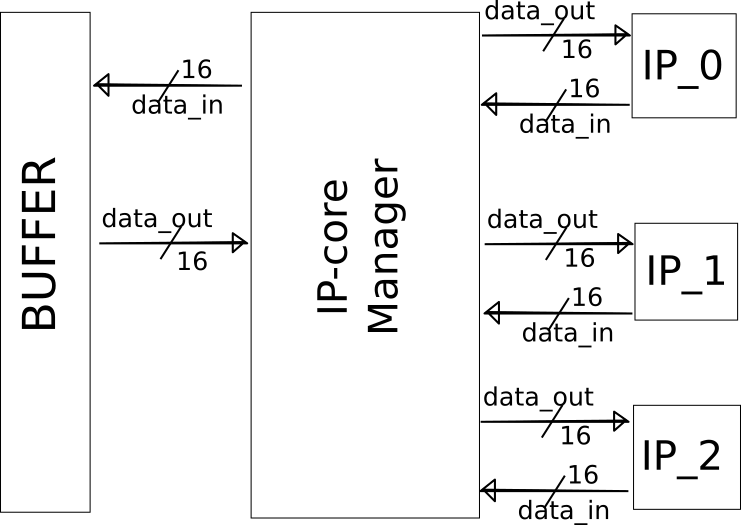
\includegraphics[width=0.9\textwidth]{imm/ip_func/x_switch.png}  
%	\caption{Cross switch} 
%	\label{fig:x_switch}
%\end{figure}

\begin{figure}[h!]
	\centering	
	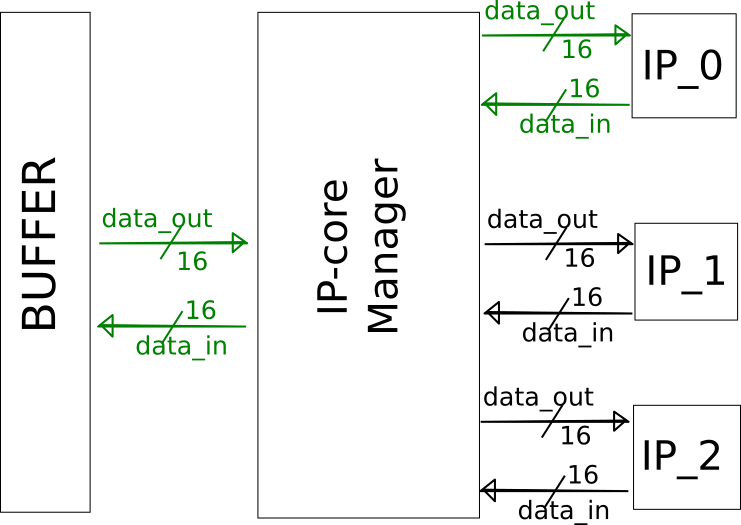
\includegraphics[width=0.85\textwidth]{imm/ip_func/x_switch22.png}  
	\caption{connecting the signal with $ IP0 $, supposing $ row_0 $ ask for the first IP core} 
	\label{fig:x_switch1}
\end{figure}
\bigskip

\begin{figure}[h!]
	\centering	
	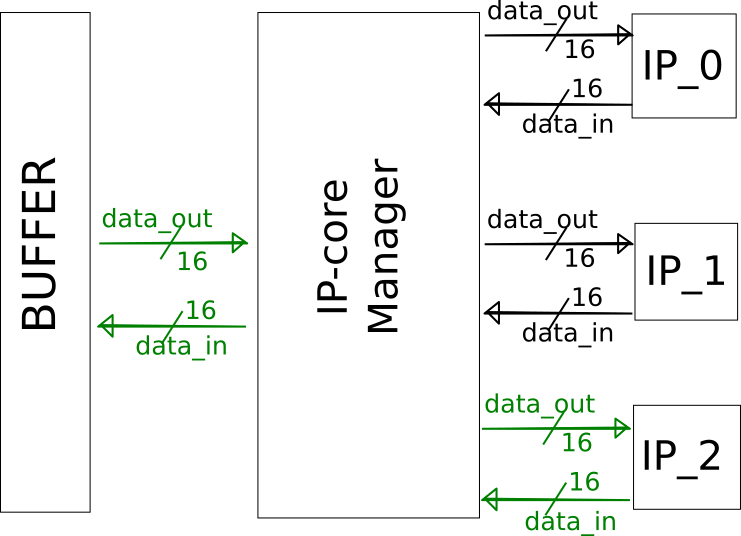
\includegraphics[width=0.85\textwidth]{imm/ip_func/x_switch33.png}  
	\caption{connecting the signal with $ IP2 $ supposing $ row_0 $ ask for the third IP core} 
	\label{fig:x_switch2}
\end{figure}

\clearpage
\section{Interrupt Handler}
The IP-core manager has to manage the case when a single or multiple core raise an interrupt request. 
However since the architecture is a master (CPU) slave (FPGA) architecture, the IP manager must guarantee that an interrupt request from one or more of IPs do not interrupt a transaction started by the master. In order words, the interrupt handler will be active at the end of a transaction.\\
In the case when multiple core raise the interrupt, the IP core manager will give priority to the core with the most priority level which is connected to the lowest port i.e. $ port_0 $.\\
In order to do so, we collect all the $ interrupt_x $ signals of the cores into an array. Than we search for the LSB at \textit{'1'}. Finally we convert the position of this bit into the physical address of the core requesting the interrupt.\\

\begin{figure}[h!]
	\centering	
	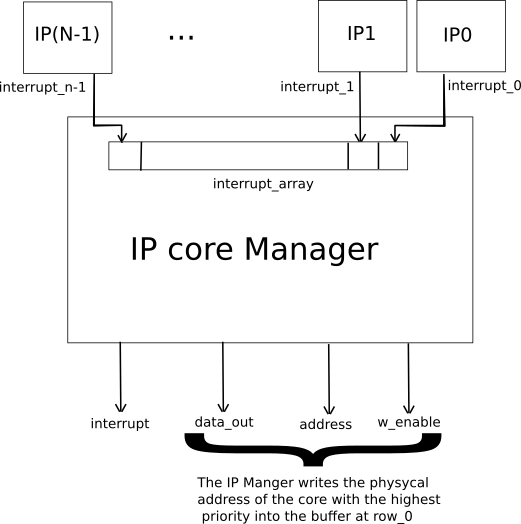
\includegraphics[width=0.85\textwidth]{imm/ip_func/interrupt.png}  
	\caption{Interrupt Handler} 
	\label{interrupt}
\end{figure}
The work of the IP Manager is first to check if there is any interrupt, this can be done by comparing the value of the interrupt vector. If the value is zero, that means that nobody raised the interrupt.\\
Otherwise it has to find the core with the highest priotiy.\\
In order to do so, it can iterate \textit{N} times, i.e. from $ i=N-1 $ to $ i=0 $. In this loop it checks the bit in \textit{Interrupt\_array(i)}, if it is $ '1' $, then the variable $ i $ is the physical address of the IP core requesting an interrupt. However, we keep the loop, because it is possible to have an IPcore with an higher priority.
\begin{figure}[h!]
	\centering	
	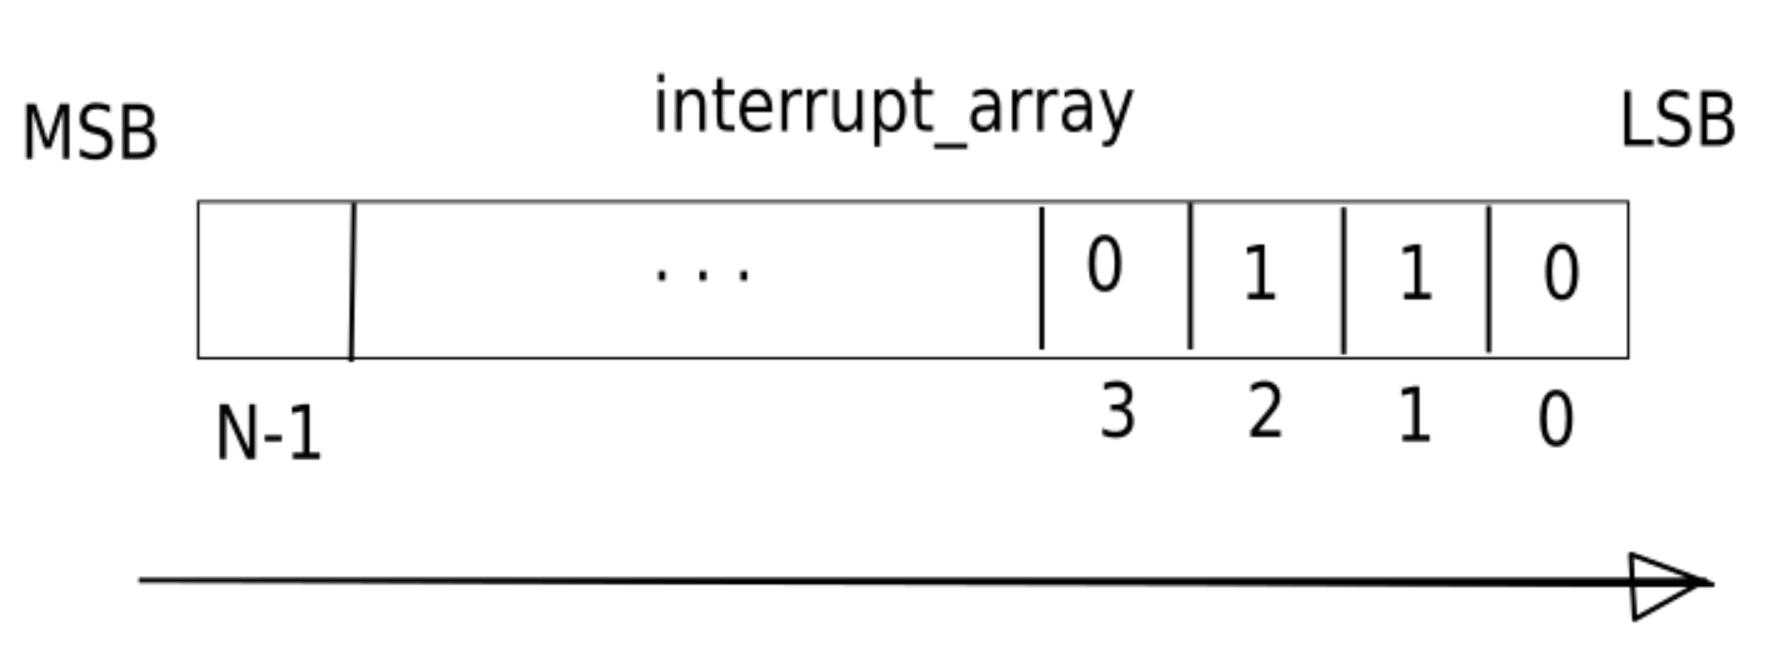
\includegraphics[width=0.85\textwidth]{imm/ip_func/int_vector.png}  
	\caption{A possible interrupt vector} 
	\label{int_vector}
\end{figure}\\
For instance, let's take the interrupt vector shown in fig. \ref{int_vector}.\\
When iterating with $ i=2 $, we wants to send the address of the third core, but when we decrease the counter $ i=1 $, we have to update this address. When $ i=0 $ we leave everything unchanged.
 
\chapter{User Manual}\label{usecase}

\section{Introduction}
The IP-core manager is an interface for the integration of multiple custom IP designs in the secube platform. It handles context switching, interrupt handling and scheduling, guaranteeing the correct exchange of data between the target IP and the CPU.
\vspace{0.5cm}\\
This guide describes the interface of the IP core manager, and is meant to assist developers and hardware designers in correctly implementing custom IP cores as well as the software that interacts with them.


%\section{Feature overview}
%CPU-initiated transactions (only one IP enabled at a time)\\
%Buffered R/W data flow\\
%Interrupt functionality\\


\section{Interface to the CPU}

The CPU talks to the IP-Core manager by the means of the data buffer. In the picture \ref{00fig}, you can see the interface of the Data buffer connected to the CPU.\\


After the cores are synthesized and running, the CPU can enable or disable the cores, load input data into them and read their output through the IP manager.
\vspace{0.5cm}\\
To do this, the CPU must initiate a transaction when it is ready to exchange data with a chosen core. 


\subsection{Initiating a transaction} \label{3.1}
Initiate or end a transaction by writing a 16-bit data packet at address row 0.\\To begin the transaction, bit 12 must be set (=1); to end the transaction, it must be unset (=0).
	\begin{center}
		\begin{tabular}{ | l | l |  l | l | }
			
			15  \qquad  \qquad 14 & 13 & 12 & 11 \qquad \qquad 0 \\ \hline
			UNUSED & INT & B/E & IP ADDR\\ \hline
			
			
			\hline
		\end{tabular}
	\end{center}
\begin{center}
	\begin{tabular}{ | c | p{7 cm} |  l |}
		\hline
		Bit(s) & Purpose & Value(s)  \\ \hline
		Bit 15 & unused  & unused 
		\\ \hline
		Bit 14 & unused  & unused\\
		\hline
		Bit 13 & Interrupt ACK from the CPU   & Normal = 0, Interrupt  =  1
		\\ \hline
		
		Bit 12 & Signals the begin/end of a transaction & Begin  = 1, End = 0 
		\\ \hline
		
		
		
		Bit 11-0 & The physical address of the target IP &
		From 0 up to N-1  \\
		
		
		
		\hline
	\end{tabular}
\end{center}
\vspace{0.5cm}
Specify the address of the target IP. Addresses are assigned sequentially from 1 to N.
\vspace{0.5cm}\\
To write the data packet, set the signals as follows:\vspace{0.5cm}\\
	\begin{tabular}{ p{0.7cm} p{14 cm} }
		&\textit{Data}: your instruction packet in the above format\\
&\textit{Address}: 0\\
&\textit{W\_enable}: 1\\
&\textit{R\_enable}: 0 \\
&\textit{Generic\_en}: 1
\end{tabular}\vspace{0.5cm}\\
\textbf{NOTE}: \textit{generic\_en} must be set to 1 whenever communication with the IP manager is in progress.\vspace{0.5cm}\\
\textbf{NOTE}: only one IP can be enabled at any time. If a new IP is enabled, all other IPs will be disabled, even if their transaction was not explicitly closed.


\subsection{Writing data to the IP core} \label{3.2}

Once a core is selected, the IP manager becomes transparent to read/write operations between core and CPU. Each core has access to a range of addresses which is freely assigned by the IP core's designer. Then, it is simply a matter of reading and writing to these addresses according to the specifications of the selected core.\vspace{0.5cm}\\
To write data, set the signals as follows:\vspace{0.5cm}\\
\begin{tabular}{ p{0.7cm} p{14 cm} }
& \textit{Data}: the 16-bit data to be sent\\
&\textit{Address}: the IP's read address (refer to the IP core's documentation)\\
&\textit{W\_enable}: 1\\
&\textit{R\_enable}: 0 \\
&\textit{Generic\_en}: 1
\end{tabular}

\subsection{Reading data from the IP core} \label{3.3}

To write data, set the signals as follows:\\
\vspace{0.5cm}
\begin{tabular}{ p{0.7cm} p{14 cm} }\\
&\textit{Data}: don't care\\
&\textit{Address}: the IP's write address (refer to the IP core's documentation)\\
&\textit{W\_enable}: 0\\
&\textit{R\_enable}: 1\\
&\textit{Generic\_en}: 1\end{tabular}

\subsection{Ending a transaction} \label{3.4}
To end a transaction, follow the steps in \ref{3.1}, and set bit 12 of the instruction packet to 0. The IP core will be unselected and disabled.


\subsection{Servicing interrupts} \label{3.5}
The CPU can receive  interrupt requests from the cores. In this event, the \textit{interrupt} signal will be raised. The IP manager will only forward interrupts when no transactions initiated by the CPU are currently active. The address of the IP requesting the interrupt is written in address row 0 by the IP manager.
\vspace{0.5cm}\\
When the CPU is ready to service an interrupt, perform the following steps:
\begin{enumerate}
\item Read address row 0 to find out the address of the requesting core.
\item Start a new transaction, selecting the requesting IP. Follow the steps in \ref{3.1}, with the only difference being that bit 13 of the control word must be set to 1. This is the ACK bit.
\item The IP core will now perform its routines. Refer to the IP core's documentation.
\item The transaction can be closed as in \ref{3.4}.
\end{enumerate}



\section{Interface to the IP cores}\label{4}

IP cores designed for the multi-IP core system must comply to the interface described in section \ref{IPinter} (see figure \ref{00fig}).\\
Note that the maximum number of IPs that can be managed by the system is $ 2^{12} $. Addresses are assigned sequentially from $ 1 $ to $ N = 2^{12} $.\vspace{0.5cm}\\
The IP cores have at their disposal the system's clock and reset signals. It is recommended that the IP's processes are made sensitive to the enable signal and that a suitable idle routine is written for when the core is disabled.\vspace{0.5cm}\\
When the core is enabled, it can perform read and write operations. When the core is disabled, it can send interrupts to the CPU to request to be enabled.


\subsection{Reading data from the cpu}\label{4.1}
When it is enabled, IP can receive data from the CPU by requesting a read from the IP manager. The range of addresses that the IP is expecting to read from can be chosen freely. However care must be taken to assign different r/w addresses to each IP in use, to avoid race conditions. The chosen addresses must be documented and communicated to the software designer.\vspace{0.5cm}\\
In order to read data, set signals as follows:\vspace{0.1cm}\\
\begin{tabular}{ p{0.7cm} p{14 cm} }\\
&\textit{address}: the IP's read address\\
&\textit{W\_enable}: 0\\
&\textit{R\_enable}: 1\\
&\textit{Generic\_en}: 1\\
\end{tabular}
\vspace{0.2cm}\\
\textbf{NOTE}: the IP manager inserts a 1-stage delay between the IP core and the CPU. The requested data will effectively appear on \textit{data\_out} with a delay of 1 clock cycle. The IP developer is invited to pipeline read requests or otherwise insert idle cycles to keep this delay into account.
\subsection{Writing data to the cpu} \label{4.2}
The write address for the core can also be freely assigned, with the same caveats as in \ref{4.1}. \vspace{0.5cm}\\To write data, set the signals as follows:\vspace{0.1cm}\\
\begin{tabular}{ p{0.7cm} p{14 cm} }\\
	&\textit{Data\_in}: the data to be written\\
&\textit{Address}: the IP's write address\\
&\textit{W\_enable}: 1\\
&\textit{R\_enable}: 0\\
&\textit{Generic\_en}: 1\\
\end{tabular}

\subsection{Requesting an interrupt} \label{4.3}
When the core is disabled, it is not able to read or write to the buffer. Then, it can send interrupts to the CPU to request to be enabled. The IP manager will only consider interrupt requests one at a time, and it assigns a static priority to the IPs according to their address; the lowest address has the highest priority. \\
\bigskip
To request an interrupt, raise the "interrupt" signal. The signal should remain high until the ACK signal is raised by the IP manager.\\ 
\bigskip
Once the CPU is ready to service the interrupt and no interrupts with higher priority are active, the IP manager will raise the \textit{ack} signal. At the same time, the IP's select signal becomes high. When the IP receives the ACK, it should unset the interrupt signal; then it can perform its operations as during a normal transaction.




\section{Use case scenario}


\subsection{Example 1: adder IP}

A user develops a simple adder. The adder receives two operands from the CPU, adds them, and delivers the result back to CPU. \\

The following buffer positions are reserved for the adder:
\begin{itemize}
\item Address row 1: OP1 
\item Address row 2: OP2
\item Address row 3: Result
\end{itemize}

The CPU writes the operands to rows 1 and 2, then enables the core, selecting IP address 1.\\

The adder core is an FSM cycling through a few states:
\begin{enumerate}
	\item \textbf{IDLE}: This state is entered at reset, and the adder stays in \textit{IDLE} whenever enable = 0. In this state, the core continuously requests to read OP1 from address row 1; this way one clock cycle is gained when starting operation since one of the operands has already been requested.

	\item \textbf{READ\_OPERAND2} : This state is entered as soon as enable becomes 1. The core requests to read OP2 from address row 2.

	\item\textbf{ WRITE\_OPERAND1}: During this cycle, OP1 is received on data\_out and stored in a local register.

	\item \textbf{WRITE\_RESULT}: OP2 is received on data out. The adder directly computes the results and writes it to the buffer's data\_in at address row 3. After this state, the core returns to \textit{IDLE}.
\end{enumerate}
In order to complete the sum, the CPU keeps the transaction open for 4 clock cycles. After this time is elapsed, the CPU can read address row 3 and retrieve the result. 

\subsection{Example 2: accumulator IP}

A user develops a second core that accumulates the value of the data found in memory for 12 clock cycles. The accumulator should work while the transaction is off and send an interrupt when the result is ready; this operation is similar to the behavior of a sensor. This IP is used at the same time as the adder IP from example 1.\\
In order to avoid conflicts with the adder, buffer positions are allocated as follows:

\begin{itemize}
\item Address row 4: OP1 
\item Address row 5: Result
\end{itemize}


Since this core is the second to be loaded in the FPGA, it is assigned IP address 2. The CPU writes the first value to be accumulated into address 4, then selects and enables the core. \\
\bigskip

The accumulator core is an FSM cycling through states:
\begin{enumerate}

\item \textbf{IDLE}: This state is entered at reset, and the adder stays in IDLE whenever enable = 0. In this state, the core continuously requests to read OP1 from address row 4.

\item \textbf{OP\_START}: This state is entered as soon as enable becomes 1. The request to read OP1 has already been sent, but the data\_out signal is not yet ready. The IP initializes a counter to 12. 

\item \textbf{ACCUMULATE}: data\_out becomes valid, and OP1 is saved in a local register and in the accumulate register. The CPU can close the transaction.
While in this state, the IP continuously adds OP1 to the ACC register and decrements the counter every clock cycle. Only once the counter rolls down to 0, it sets interrupt to 1 and continues to state 4.

\item \textbf{WAIT\_ACK}: The interrupt has been sent on the last iteration of state 3. This state polls the ack signal every clock cycle. 
When the CPU is ready to read the result, it opens a transaction with the accumulator core while setting the ACK bit in the control packet. Once ack becomes 1, the IP sets interrupt to 0 and proceeds to state 5.

\item\textbf{ WRITE\_RES}: The result is written to address row 5. After this state, the IP returns to IDLE.

\end{enumerate}
In order to initiate operation, the CPU keeps the transaction open for 2 clock cycles to allow for the read of OP1. When reading the result, the transaction stays open for 3 clock cycles, after which the result appears in the buffer.
\chapter{Guidelines}\label{Guidelines}
\begin{itemize}
\item To reduce the latency, it's better if the synchronous IP cores start with the interface signals ``loaded'' with the address of the first data to read.
\item Another way to reduce the latency is to have the IP cores working on the falling edge of the clock instead of the rising edge like does the IP manager.
\item Synthesizer like Vivado and Lattice don't like very much asynchronous memories like our Data Buffer. Usually they automatically introduce latches. Be aware that these can introduce differences between the simulation behaviour and the behaviour on FPGA.
\end{itemize}
\chapter{Future developments}\label{future}
\section{Asynchronous is the new synchronous}
As we have seen in the previous chapters a synchronous IP manager introduces several clock cycle of latency in the overall transaction between CPU and the cores.\\
A possible future devolpment to remove this latency is to change from the current clock based, sequential implementation to a full combinational one.
\section{Configurable manager}
We have reserved the address 0 for the IP manager, in case the CPU wants to \textit{configure} it. Which possible configurations are available? None! That's up to you to implement it. 
\section{Interface for the IP cores}
Every IP in the world is designed with a custom interface, and they are usually all different.\\
A possible future developments is to analyze if it is possible to realize an hardware component capable of adapting whatever IP interface to the interface compliant with this architecture and described in this document.
% \input{./chapters/chap_name}
% and so on
%
%%%%%%%%%%%%%%%%%%%%%%%%%%%%%%%%%%%%%%%%%%%%%%%%%%%%%%
%    
% HERE IS WHERE YOU INCLUDE YOUR APPENDICES (IF ANY)
%
%\appendix
%%%% Appendix A
\chapter{Adder behavioural VHDL}
\label{appendix1}

	\lstinputlisting[language=VHDL, breaklines=true]{appendices/files/adder.vhd}

% \lstinputlisting is an alternative way to import text or code from an external file. In this example the behavioural VHDL description of an adder contained in the file adder.vhd is imported. 
% Note that you can set the language of the code that you want to import (VHDL in this example). When you set the language you will see the keywords of that specific language highlighted in your output pdf file.
%You can set a lot parameters: for some examples take a look at the chapter 'How to document the project' that can you find in DLX_Project.pdf.
% \input{./appendices/appendix2}
% and so on
%
%%%%%%%%%%%%%%%%%%%%%%%%%%%%%%%%%%%%%%%%%%%%%%%%%%%%%%

\end{document}